\documentclass[12pt]{beamer}
\usetheme{CambridgeUS}

\usepackage{amssymb,amsmath, amsfonts, graphicx, wasysym, moresize}

\graphicspath{{images/}}

\newcommand\blfootnote[1]{%
  \begingroup
  \renewcommand\thefootnote{}\footnote{#1}%
  \addtocounter{footnote}{-1}%
  \endgroup
}

\title{Heterogeneity in Returns to College Major}

\author{By Oliver Titus \\
\and Sponsored by Dr. Marr (EHPS)}
\date{April 18, 2019}
\begin{document}
\begin{frame}
\titlepage

\includegraphics[scale=0.1]{logo.jpg}
\end{frame}

\begin{frame}
\frametitle{Motivation}
\begin{itemize}
\item Many choose their college major based on the following:
\begin{itemize}
\item Expectations of future earnings
\item Preferences
\item Ability and preparation
\end{itemize}
\item About 35 percent of today's jobs require a Bachelor's degree or higher.
\item Recent college graduates' annual wages vary from \$27,000 to \$50,000 depending on major choice.
\item Used 2009 American Community Survey data to answer the following questions:
\begin{itemize}
\item How do different fields of bachelor's degree affect hourly wage outcomes?
\item How do wage outcomes differ by gender?
\end{itemize}
\end{itemize}
\end{frame}

\begin{frame}
\frametitle{Literature}
\begin{itemize}
\item Altonji, Blom, and Meghir (2012) used the same data set to analyze labor market returns on college major and high school coursework.
\item Daymont and Andrisani (1984) used data from the National Longitudinal studies of the High School Class of 1972 to analyze the gender gap in earnings among recent college graduates.
\item Georgetown University (2015) used Census Data to analyze wages for 137 college majors.
\end{itemize}
\end{frame}

\begin{frame}
\frametitle{Summary Statistics}
\begin{center}
\begin{table}
\resizebox{\columnwidth}{!}{%
\begin{tabular}{|c | c c c c|}
\hline
\textbf{Variable} & \textbf{Mean} & \textbf{Std. Dev.} & \textbf{Min} & \textbf{Max} \\
\hline
Age &   42.862   &  15.293     &    16    &     70\\
Education &   17.852  &  3.522   &       1  &       24 \\
Income &    36408.34  &  51561.21  &   0  &  1288000 \\
Annual Hours Worked &  1778.78  &  793.21     &    7    &   5049 \\
Hourly Wage   &  22.49  &  78.2   &       0  & 53571.43 \\
\hline
\end{tabular}%
}
\blfootnote{\textbf{n}=1270870}
\end{table}
\end{center}
\end{frame}

\begin{frame}
\frametitle{Top 5 Majors Categories for Each Gender}
\begin{table}[t]
\caption{Top 5 Male Dominated Major Categories}
\centering
\resizebox{.35\columnwidth}{!}{%
\begin{tabular}{|c| c|}
\hline
\textbf{Major Category} & \% \textbf{Male} \\
\hline
Business & 56 \\
Social Sciences & 52 \\
Engineering & 65 \\
Science & 56 \\
Computers & 80 \\
\hline
\end{tabular}%
}
\end{table}
\begin{table}[b]
\caption{Top 5 Female Dominated Major Categories}
\centering
\resizebox{.45\columnwidth}{!}{%
\begin{tabular}{|c| c|}
\hline
\textbf{Major Category} & \% \textbf{Female} \\
\hline
Education & 76 \\
Medical/Health Services & 84 \\
Liberal Arts & 69 \\
Psychology & 69 \\
Art & 63 \\
\hline
\end{tabular}%
}
\end{table}
\end{frame}

\begin{frame}
\frametitle{Income Dispersion by Major}
\begin{center}
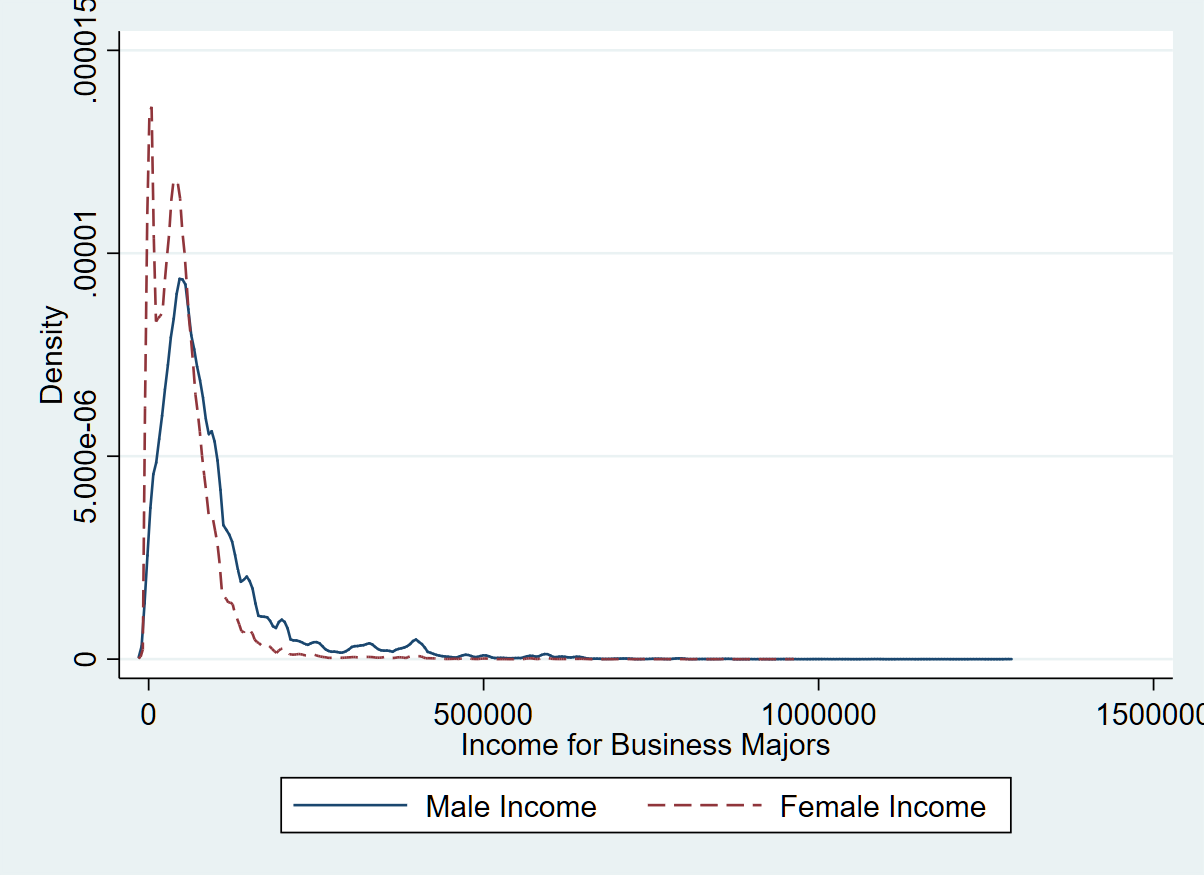
\includegraphics[scale=0.1395]{business.png}
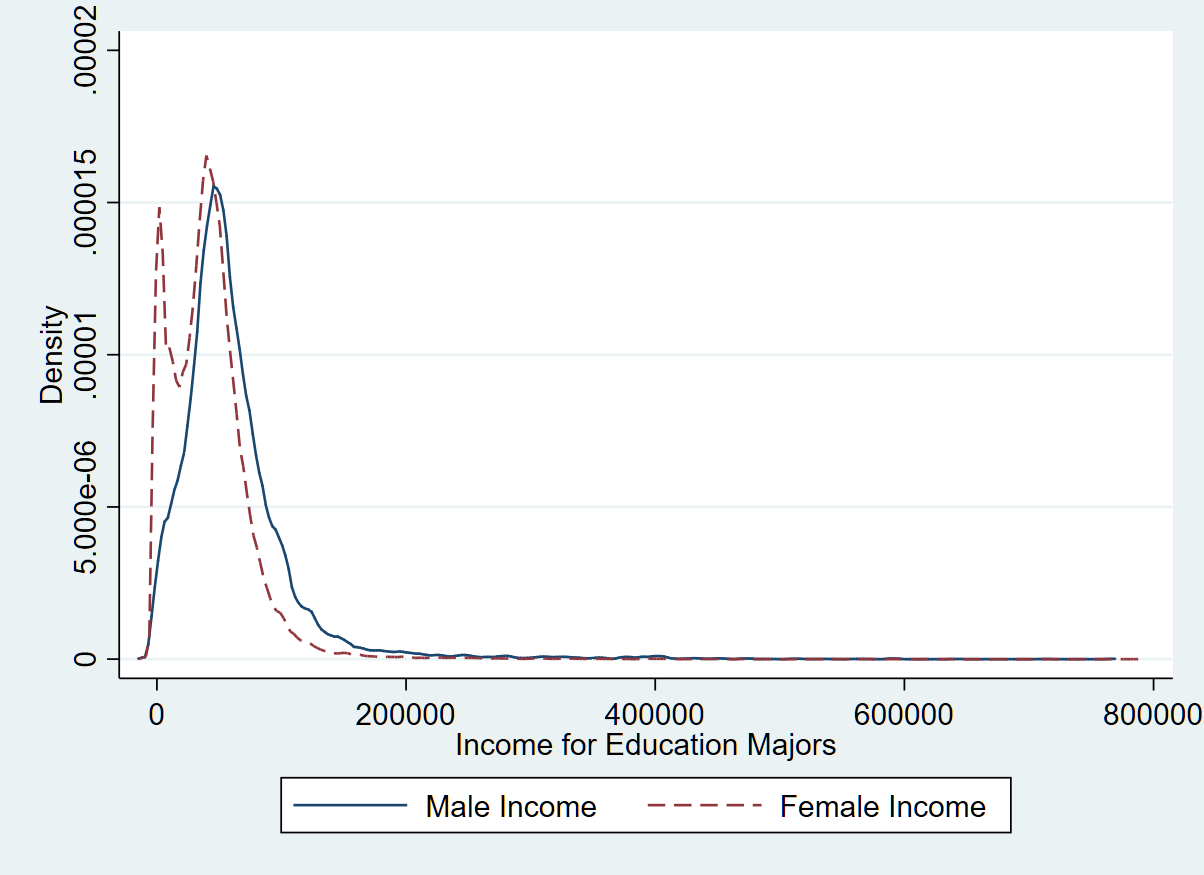
\includegraphics[scale=0.1395]{education.png}
\end{center}
\end{frame}

\begin{frame}
\frametitle{Specification}
Consider the wage equation:
\begin{equation}
\ln(Y_i) = \beta_0 + \beta_1 X_i + \beta_2 E_i + \beta_3 R_i + \beta_4 F_i + \beta_5 M_i + \epsilon_i
\end{equation}
\begin{itemize}
\item $Y_i$ is the hourly wage.
\item $X_i$ is the set of major dummies with Business Majors being set as the base.
\item $E_i$ is higher degree levels including masters, professional degree, and PhD.
\item $R_i$ is the set of races.
\item $F_i$ is a female dummy variable.
\item $M_i$ is dummy variable that denotes marital status.
\item $\epsilon_i$ is other factors not accounted for.
\end{itemize}
\end{frame}

\begin{frame}
\frametitle{Results: Wage Heterogeneity}
\begin{itemize}
\item This table compares hourly wages to the hourly for Business Majors. Business Majors have a mean hourly wage \$36.15 per hour.
\end{itemize}

\begin{table}
\centering
\resizebox{.9\columnwidth}{!}{%
\begin{tabular}{| c | c | c | c |}
\hline
\textbf{Major} & \textbf{Full Sample (\$)} & \textbf{Males Only (\$)} & \textbf{Females Only (\$)} \\
\hline
No bachelor's degree & -15.65*** & -18.28*** & -11.57*** \\
Computers & 0.83 & -1.59 & 4.47*** \\
Mathematics & 2.12** & 1.78 & 2.38*** \\
Education & -9.99*** & -12.38*** & -5.53*** \\
Engineering & 5.07*** & 2.33*** & 7.05*** \\
Liberal Arts & -8.30*** & -9.05*** & -4.98*** \\
Medical/Health Services & -0.94* & -1.10 & 2.86*** \\
Philosophy and Religion & -15.88*** & -20.05*** & -9.27*** \\
Psychology & -9.23*** & -9.59*** & -6.09*** \\
Social Sciences & -4.13*** & -4.31*** & -3.32*** \\
\hline
\end{tabular}%
}
\blfootnote{***p $<$ 0.01 **p $<$ 0.05 *p $<$ 0.1}
\blfootnote{\textbf{Note:} Female dummy had a coefficient of -5.06 in the full sample.}
\end{table}
\end{frame}

\begin{frame}
\frametitle{Results: Female Wage Differences}
\begin{itemize}
\item To test for wage heterogeneity for gender by major, I run the following regression:
\begin{equation}
\ln(Y_i) = \beta_0 + \beta_1F_i + \beta_2X_i + \beta_3X_i*F_i + \epsilon_i
\end{equation}
\end{itemize}
\begin{table}
\resizebox{.69\columnwidth}{!}{%
\begin{tabular}{|c |c|}
\hline
\textbf{Major} & \textbf{Female Hourly Wage Difference (\%)} \\
\hline
Business & -6.31*** \\
Computers & 3.82** \\
Mathematics & -6.21*** \\
Education & 9.15*** \\
Engineering & 0.62 \\
Liberal Arts & -1.98** \\
Medical/Health Services & -0.93 \\
Philosophy and Religion & 11.03*** \\
Psychology & -4.70*** \\
Science & -13.76*** \\
Art & 5.31*** \\
\hline
\end{tabular}%
}
\begin{footnotesize}
\blfootnote{***p $<$ 0.01 **p $<$ 0.05 *p $<$ 0.1}
\blfootnote{\textbf{Note:} Female dummy had a coefficient of -0.22 implying that females make 22\% less than men on average.}
\end{footnotesize}

\end{table}
\end{frame}

\begin{frame}
\frametitle{Conclusion}
\begin{itemize}
\item Engineering majors have the highest hourly wage returns on average.
\item Philosophy and Religion majors have the lowest hourly wage returns on average.
\item Female wages are lower the male wages in most of the majors, however Females with an Art, Education, Computer, or Philosophy major have higher wages than men with those majors.
\item A Chow Test was conducted and returned an F-statistic of 2996.41 which gives a P-value less that 0.01 implying that hourly wages are different for men and women in each major category with high statistical significance. 
\end{itemize}
\end{frame}
\begin{frame}
\begin{center}
\huge Thank you!
\end{center}
\end{frame}
\end{document}